% Cap�tulo 3


\chapter{Arquitetura do Hardware}

A arquitetura do projeto foi projetada começando de um protótipo funcional, e toda a sua parte de seleção de componentes, até uma versão estável que conseguisse solucionar o cubo perfeitamente.


\section{Protótipo Inicial}

Como primeira parte do projeto, temos o  desenvolvimento de um protótipo para testes, definição de medidas e ângulos que o robô deve ter para possibilitar a resolução completa do cubo mágico. Essa versão inicial, foi construída com palitos de picolé como mostrado na figura.

\begin{figure}[htb]
	\centering
  	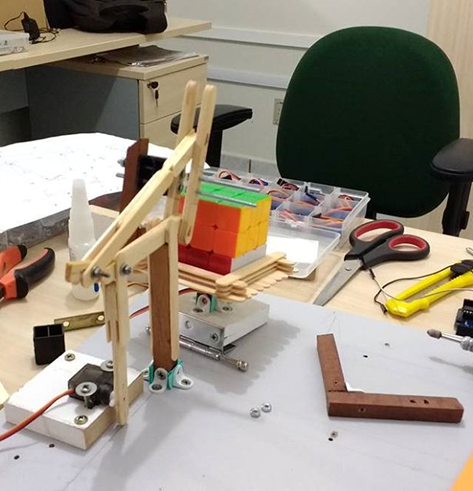
\includegraphics[scale=0.40]{imagens/prototipo.png}
  	\textsf{\caption{Protótipo para testes }}
  	\label{fig:FiguraTeste}
\end{figure}

Nessa fase de prototipagem, foram feitos testes com equipamentos diferentes para selecionar os componentes de hardware necessários. Ao garantir o funcionamento dos componentes em posições específicas testadas com o protótipo, é iniciado a  construção da versão final e a programação destes componentes.


A estrutura de hardware do robô é composta por peças feitas com o auxílio da impressora 3D em material específico para a impressão, uma base para o cubo, um braço de movimento horizontal, e uma garra que ajusta o cubo. Esses materiais estão dispostos em uma área medindo 49.5cm de comprimento e 15cm de largura. O cubo usado para o projeto é o Shengshou Stickerless modelo Rainbow Stickerless 3X3. O funcionamento do robô consiste em o braço mecânico empurrar o cubo para mudar para face seguinte, e para trocar as peças de face, o braço segura o cubo enquanto a base gira 90, 180 ou 360 graus. Em seguida, a garra de ajuste nivela o cubo. 

    \begin{figure}[htb]
	\centering
  	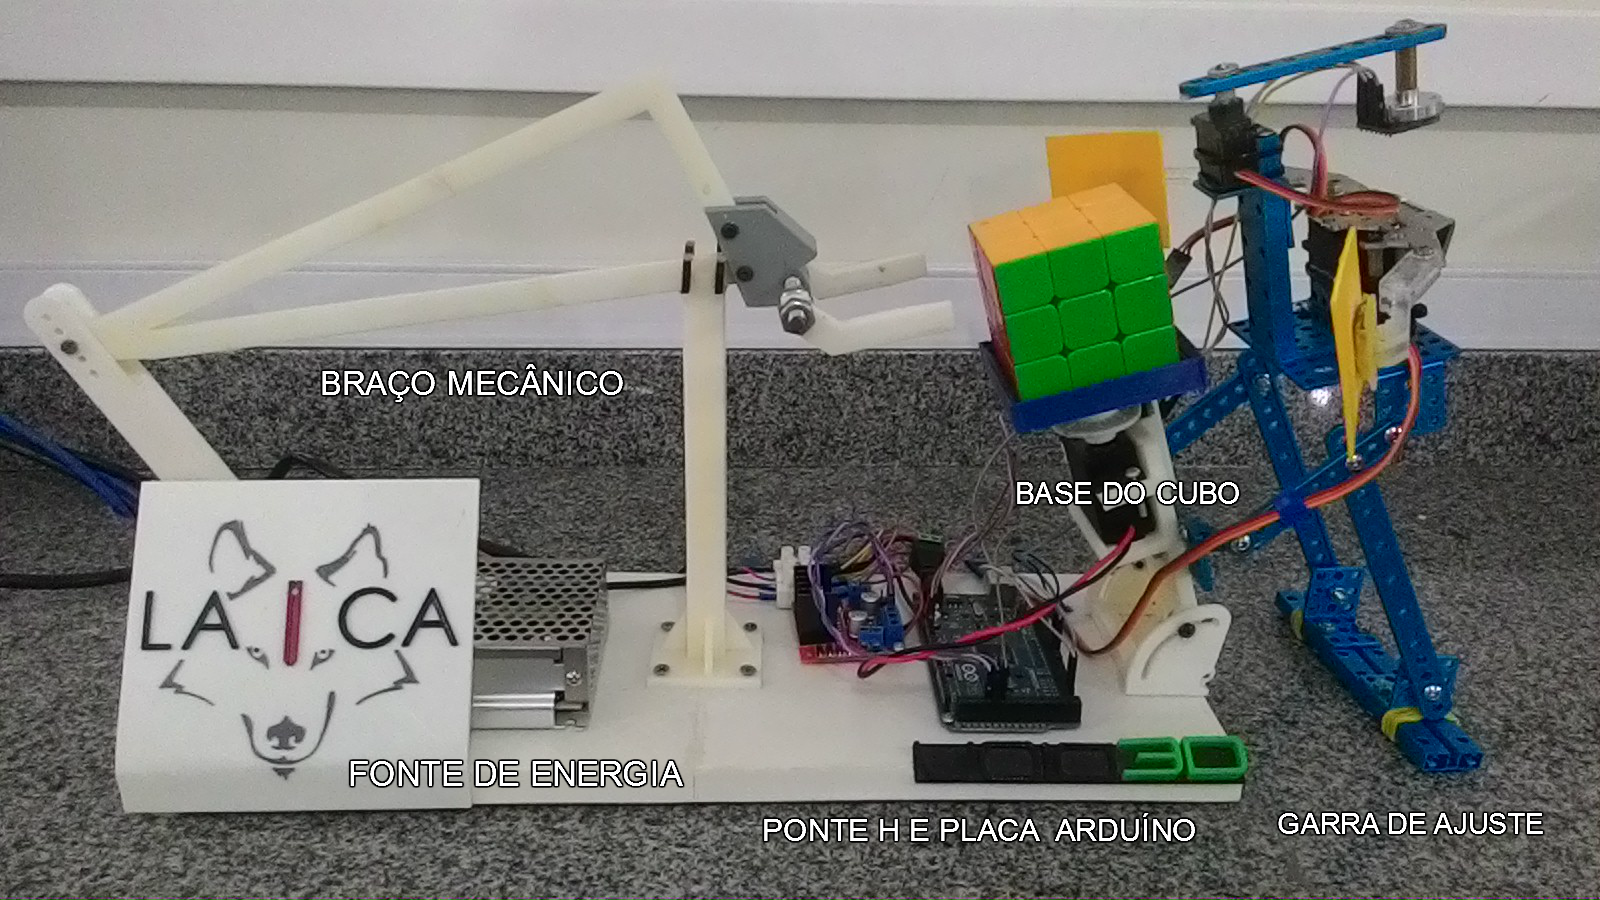
\includegraphics[scale=0.20]{imagens/robo.png}
  	\textsf{\caption{Robô que soluciona o cubo }}
  	\label{fig:FiguraTeste}
\end{figure}


\section{Braço Mecânico}

O braço mecânico de movimento horizontal, é movimentado por meio de um servo motor TowerPro modelo MG99.
\begin{figure}[htb]
	\centering
  	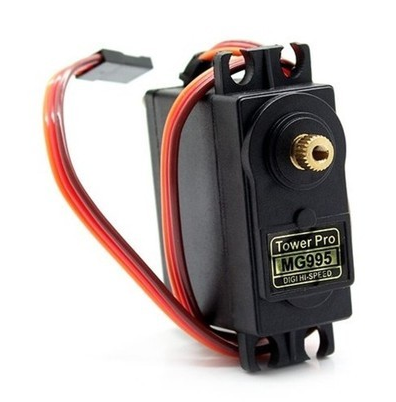
\includegraphics[scale=0.45]{imagens/servo1.png}
  	\textsf{\caption{Servo motor modelo TowerPro }}
  	\label{fig:FiguraTeste}
\end{figure}
 Esse servo se movimenta por meio de um algoritmo que é composto por quatro funções, são elas uma responsável por parar o movimento do servo quando necessário e outras três para movimentar o braço nas posições 90,  50 e 20 graus.
 
 Em relação às funções relacionadas ao servo, a função usada para parar o servo pode ser vista no código abaixo:
 
 \begin{algorithm}[H]
   \SetAlgoLined
   \Inicio{
   \begin{enumerate}
   
   \item analogWrite(ena, 255)
   
   \item digitalWrite(in1, HIGH)
   
   \item digitalWrite(in2, HIGH)
    \end{enumerate}
   }
   \label{alg1}
   \caption{\textsc{Parar}}
 \end{algorithm}
 
 
 
 A função \textit{analogWrite} é usada para definir a porta 255 do arduíno para a ponte H, referenciada no algoritmo pela variável ENA(variável padrão para setar a velocidade máxima no motor), enquanto as funções \textit{digitalWrite} são usadas para passar voltagem ao mesmo tempo, por meio das variáveis in1 e in2, para o servo fazendo com que ele pare. Para colocar o braço mecânico na posição inicial de 90 graus é usada a função mostrada abaixo:
 

 \begin{algorithm}[H]
   \SetAlgoLined
   \Inicio{
   \begin{enumerate}
   \item digitalWrite(servo\_garra, HIGH)
   \item delayMicroseconds(1200)
   \item digitalWrite(servo\_garra, LOW)
   
   
   
   \item \Para{i==0 até 15}{
   \item delayMicroseconds(1200)} 
   \EndFor
    \end{enumerate}
   }
   \label{alg1}
   \caption{\textsc{Servo90graus}}
 \end{algorithm}
 
 
 Essa função é composta por:  \textit{digitalWrite(servo\_garra, HIGH), (iv) delayMicroseconds(1200),  digitalWrite(servo\_garra, LOW) e \ for(int i=0; i<15; i++) delayMicroseconds(1200)}. Definimos uma variável chamada servo\_garra para a porta do arduíno na qual está conectada o servo. As funções \textit{digitalWrite} são responsáveis por passar voltagem para o servo ou parar a voltagem quando necessário, e com as \textit{delayMicroseconds}, estabelecemos um tempo definido em segundos para que o servo fique parado. Também usamos o \textit{for(int i=0; i<15; i++) delayMicroseconds(1200);} para prolongar o tempo de espera do servo.
 
Para posicionar o servo no ângulo de  50 graus, que corresponde a posição para segurar o cubo, é usada a função abaixo:
\begin{algorithm}[H]
   \SetAlgoLined
   \Inicio{
   \begin{enumerate}
   \item digitalWrite(servo\_garra, HIGH)
   
   \item delayMicroseconds(930)
   
   \item digitalWrite(servo\_garra, LOW)
   
   \item \Para{i==0 até 20}{\item delayMicroseconds(930)} 
  \EndFor
  
  \end{enumerate}
    
   }
   \label{alg1}
   \caption{\textsc{Servo50graus}}
 \end{algorithm}



Essa função é composta por:  \textit{digitalWrite(servo\_garra, HIGH),  delayMicroseconds(930),  digitalWrite(servo\_garra, LOW) e for(int i=0; i<20; i++)  delayMicroseconds(930)}. Diminuímos o tempo de espera do servo para que o braço mecânico consiga alcançar o cubo. A última função é responsável por posicionar o servo no ângulo de 20 graus, para que o braço mecânico empurre o cubo.

\begin{algorithm}[H]
   \SetAlgoLined
   \Inicio{
   \begin{enumerate}
   \item digitalWrite(servo\_garra, HIGH)
   
   \item delayMicroseconds(760)
   
   \item digitalWrite(servo\_garra, LOW)
   
    \item \Para{i==0 até 25}{\item delayMicroseconds(760)} 
  \EndFor
    \end{enumerate}
   }
   \label{alg1}
   \caption{\textsc{Servo20graus}}
 \end{algorithm}




Essa função é composta por:  \textit{digitalWrite(servo\_garra, HIGH), delayMicroseconds(760),  digitalWrite(servo\_garra, LOW) e for(int i=0; i<25; i++) delayMicroseconds(760)}. Para que o braço empurre o cubo, o tempo de espera do servo é diminuído fazendo com que ele se mova mais para frente, empurre o cubo e volte para a posição inicial.

\section{Base do cubo}

 \begin{figure}[htb]
	\centering
  	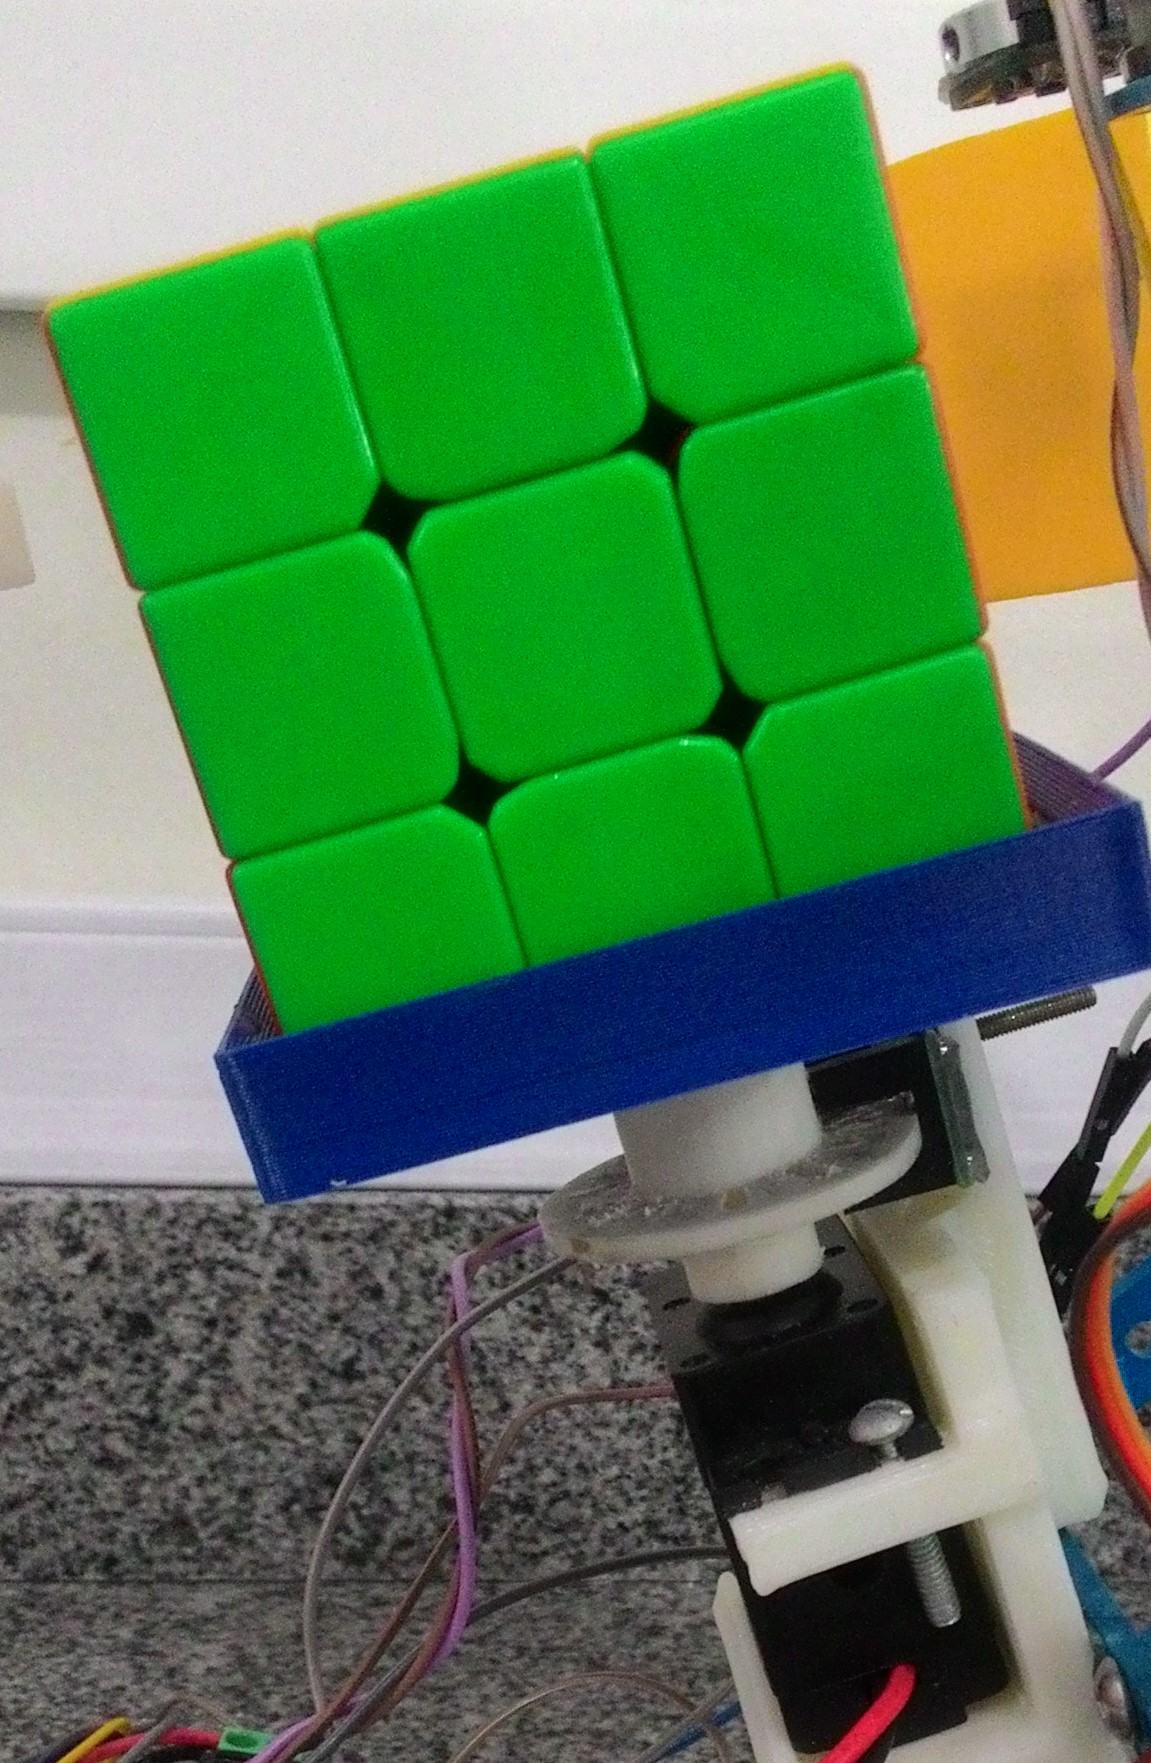
\includegraphics[scale=0.1]{imagens/base.jpg}
  	\textsf{\caption{Base do cubo}}
  	\label{fig:FiguraTeste}
\end{figure}

    A base do cubo é uma peça construída com a impressora 3d, medindo 6.7 cm de largura e 6.7 cm de altura, e é responsável por girar o cubo nas posições 90, 180 e 360 graus. Ela se movimenta por meio do servo TowerPro. Para realizar esses movimentos, também é necessário um encoder óptico de 5mm e um disco rotativo. O encoder é dispositivo eletromecânico que conta ou reproduz pulsos elétricos a partir do movimento rotacional de seu eixo. A cada volta do disco rotativo, o encoder acrescenta na contagem para saber exatamente onde parar nas posições certas.

    Para a base fazer a rotação, são usadas duas funções: \textit{anda90livre()} e \textit{anda90garra()}. A função a\textit{anda90livre()}, é responsável por girar a base em 90 graus no sentido horário quando a garra está na posição inicial.
    
    
    
\begin{algorithm}[H]
   \SetAlgoLined
   \Inicio{
   \begin{enumerate}
   \item pulso = digitalWrite(pinoDO);
   \item \While{pulso == 1 e fimmovimento == 1}{
        \item analogWrite(ena, 55);
        
        \item digitalWrite(in1, LOW);
        
        \item digitalWrtite(in2, HIGH);
        
        \item pulso = digitalRead(pinoDO);
  }
 
   \item parar();
   
   \item delay(20);
   
\item    analogWrite(ena, 50);
   
   \item digitalWrite(in1, HIGH);
   
   \item digitalWrite(in2, LOW);
   
   \item delay(54);
   
   \item parar();
   
   \item fimmovimento = 0;
   
   \item delay(500);
   \end{enumerate}
   }
   
   \label{alg1}
   \caption{\textsc{anda90livre()}}
 \end{algorithm}
    
 A variável pulso é usada para controlar a quantidade de voltas que o disco óptico faz, e por meio do bloco Enquanto, a base gira até ser passado outro valor para a variável pulso.
 
 A função \textit{anda90garra()}, é responsável por mover a base em 90 graus no sentido horário quando a garra está segurando o cubo. Assim, é possível mudar as peças do cubo de uma face para outra.
 
 \begin{algorithm}[H]
   \SetAlgoLined
   \Inicio{
   
   \begin{enumerate}
   \item pulso = digitalWrite(pinoDO);
   
   \item \While{pulso == 1 e fimmovimento == 1}{
        \item analogWrite(ena, 60);
        
        \item digitalWrite(in1, LOW);
        
        \item digitalWrtite(in2, HIGH);
        
        \item pulso = digitalRead(pinoDO);
 
 
 }
 
   \item parar();
   
   \item delay(20);
   \end{enumerate}
   }
   \label{alg1}
   \caption{\textsc{anda90garra()}}
 \end{algorithm}
   
   A função também usa a variável pulso para controlar as voltas mas usa o valor 60 na função \textit{analogWrite(ena, 60);}. Isso é feito para passar mais voltagem para a base fazendo possível seu movimento mesmo que o braço mecânico esteja segurando o cubo.

\section{Garra de Ajuste}

Para dar estabilidade a  base, existe uma estrutura de metal de 23.5 cm de altura. Na parte de cima dessa estrutura, existe um servo motor TowerPro acoplado a uma garra mecânica modelo Robot Mechanical Claw H3 modificada.  A garra é responsável por ajustar os lados do cubo quando suas peças mudam de lugar. 

\begin{figure}[htb]
	\centering
  	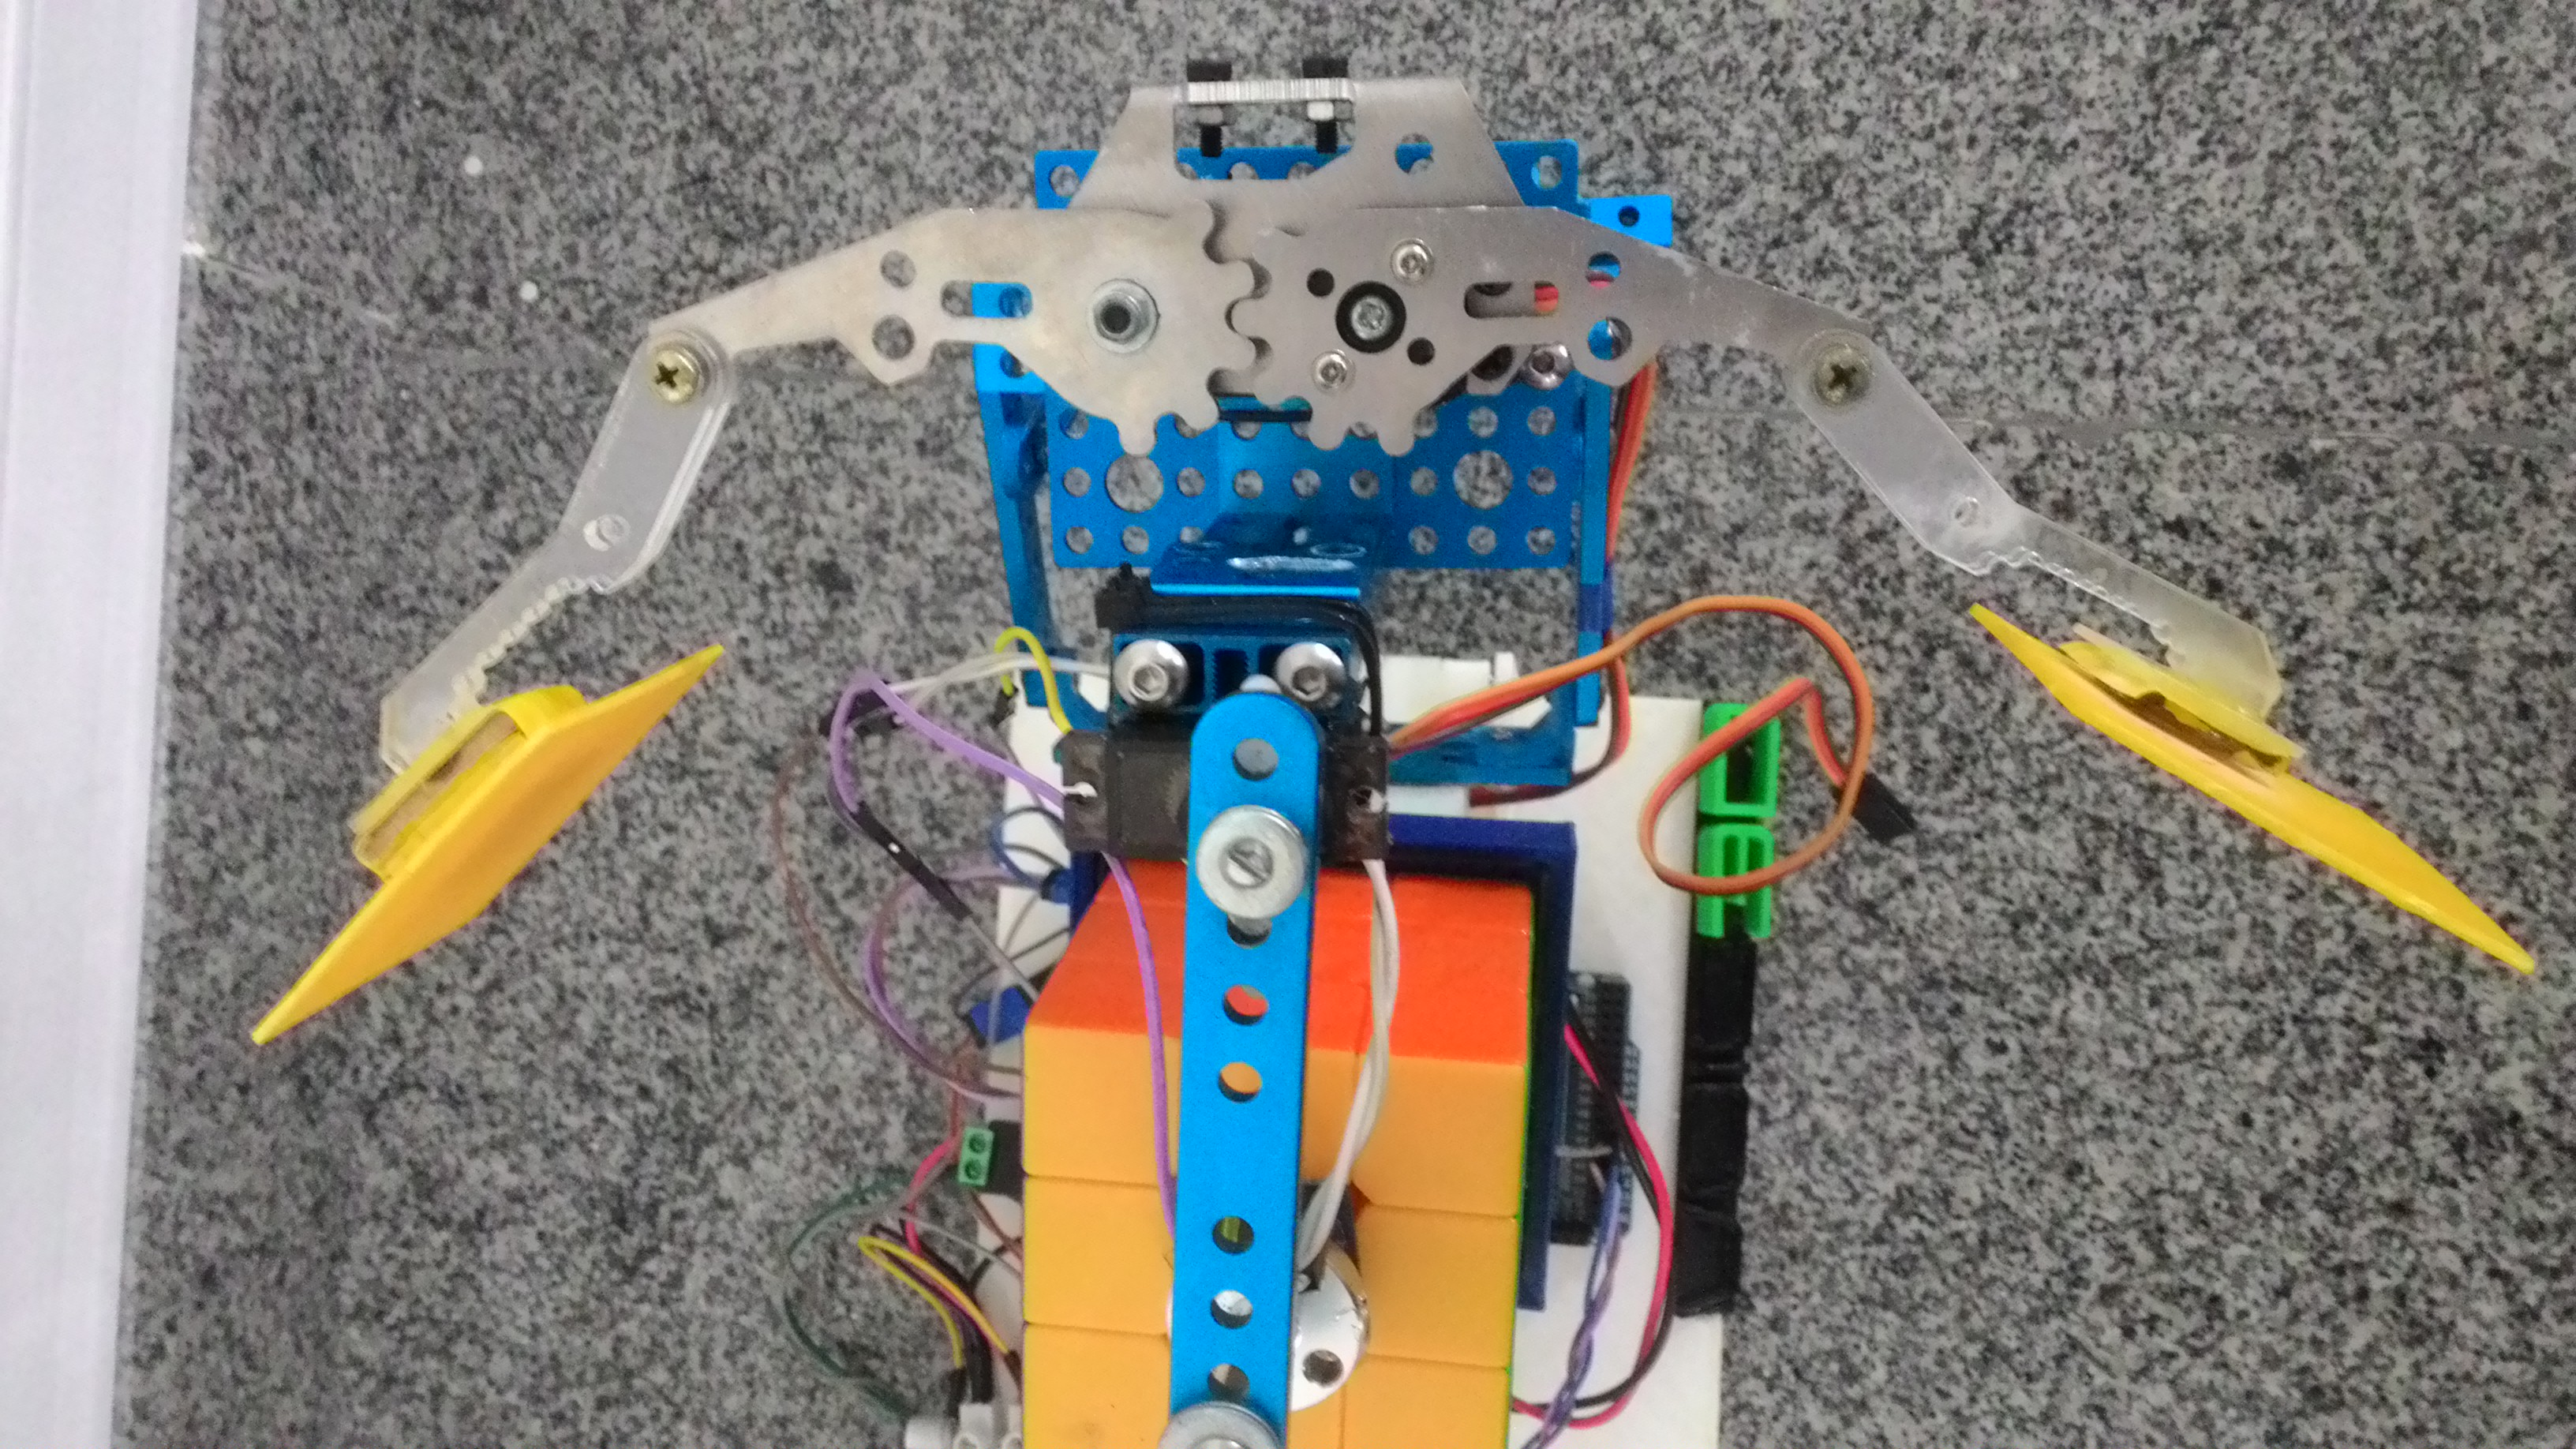
\includegraphics[scale=0.1]{imagens/garra.jpg}
  	\textsf{\caption{Garra de ajuste}}
  	\label{fig:FiguraTeste}
\end{figure}

A garra está conectada na porta porta 3 PWM(Pulse Width Modulation) do arduíno, que corresponde a alteração da largura do sinal de onda passada, e faz o movimento de fechar e abrir quando necessário por meio das funções \textit{servoajusteFechar()} e \textit{servoajusteAbrir()}.

 \begin{algorithm}[H]
   \SetAlgoLined
   \Inicio{
   \begin{enumerate}
    \item digitalWrite(servoajuste, HIGH);
    
    \item delayMicroseconds(900);
    
    \item digitalWrite(servoajuste, LOW);
 
   \item \Para{i==0 até i menor que 2}{\item delayMicroseconds(900);} 
  \EndFor
   
   \end{enumerate}}
   \label{alg1}
   \caption{\textsc{servoajusteFechar()}}
 \end{algorithm}
 
 A função \textit{servoajusteFechar()}, passa corrente para o servo por meio da função 
 \textit{digitalWrite(servoajuste, HIGH);} fazendo com que a garra feche até o ângulo adequado para ajustar o cubo definido pela função \textit{delayMicroseconds(900);}.
 
 \begin{algorithm}[H]
   \SetAlgoLined
   \Inicio{
   \begin{enumerate}
    \item digitalWrite(servoajuste, HIGH);
    
    \item delayMicroseconds(2400);
    
    \item digitalWrite(servoajuste, LOW);
 
   \item \Para{i==0 até i menor que 7}{\item delayMicroseconds(1400);} 
  \EndFor
  \end{enumerate}
   }
   \label{alg1}
   \caption{\textsc{servoajusteAbrir()}}
 \end{algorithm}
 
 
 A função \textit{servoajusteAbrir()}, passa corrente para o servo por meio da função 
 \textit{digitalWrite(servoajuste, HIGH);} fazendo com que a garra abra até sua posição original definida pela função \textit{delayMicroseconds(2400);}.



\section{Ponte H}

A função da Ponte H é controlar a velocidade e o sentido dos motores usados para construir o robô. Ela é um circuito eletrônico que permite que o micro controlador forneça a corrente necessária para o funcionamento do Motor de corrente contínua. A ponte H usada é a modelo L298N com um ST chip de L298N.

\begin{figure}[htb]
	\centering
  	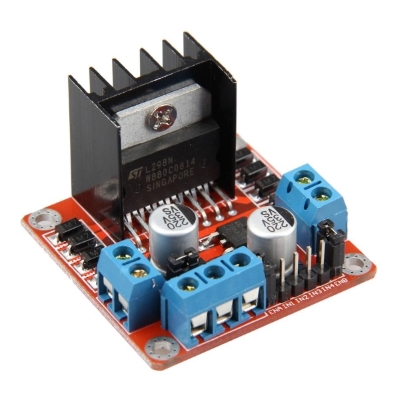
\includegraphics[scale=0.60]{imagens/ponte.jpg}
  	\textsf{\caption{Ponte H}}
  	\label{fig:FiguraTeste}
\end{figure}



A ponte H está ligada a um regulador de tensão modelo LM2596, responsável por regular a divisão de potência reativa entre os dispositivos. Para seu funcionamento é preciso definir uma configuração inicial. É alocado a variável \textit{ena(enable A)} para a porta 44 do arduíno, a variável in1 para a porta 45 e a variável in2 para a porta 46.

\begin{figure}[htb]
	\centering
  	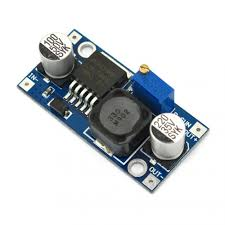
\includegraphics[scale=0.60]{imagens/regulador.jpg} 
  	\textsf{\caption{Regulador de Tensão}}
  	\label{fig:FiguraTeste}
\end{figure}



\section{Arduíno}

Todos os equipamentos citados anteriormente, estão conectados a um arduíno Mega modelo 2560. A placa possui 54 pinos de entradas e saídas digitais onde 15 destes podem ser utilizados como saídas PWM. Possui também, 16 entradas analógicas e 4 portas de comunicação serial. É usado com uma fonte externa e um cabo USB(Universal Serial Bus) para fazer conexão com o computador.

\begin{figure}[htb]
	\centering
  	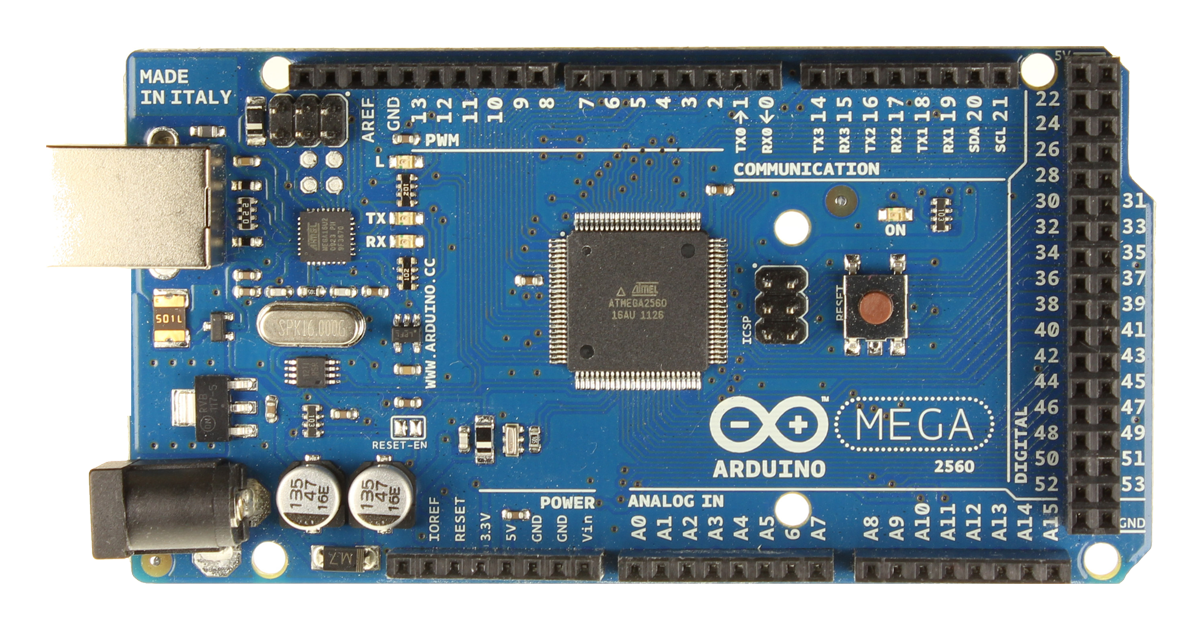
\includegraphics[scale=0.13]{imagens/arduino.png}
  	\textsf{\caption{arduíno Mega}}
  	\label{fig:FiguraTeste}
\end{figure}

Para seu funcionamento é definido uma configuração inicial por meio do código mostrado abaixo: 

 \begin{algorithm}[H]
   \SetAlgoLined
   \Inicio{
   \begin{enumerate}
    \item Serial.begin(9600);
    
    \item pinMode(servo\_garra, OUTPUT);
    
    \item pinMode(servo\_ajuste, OUTPUT);
    
    \item pinMode(pinoDO, INPUT);
 
    \item pulso = 0;
    
    \item inicio();
   \end{enumerate}}
   \label{alg1}
   \caption{\textsc{setup()}}
 \end{algorithm}
 
 A função \textit{Serial.begin(9600);} inicia a leitura dos dados. As funções \textit{pinMode(servo\_garra, OUTPUT); e pinMode(servo\_ajuste, OUTPUT);} definem o servo da garra e o servo de ajuste como saída. A função \textit{pinMode(pinoDO, INPUT);} define o  sinal do encoder como entrada, também é definido o valor 0 para a variável pulso e é chamada a função \textit{inicio()} para iniciar o programa.
 
 \begin{algorithm}[H]
   \SetAlgoLined
   \Inicio{
   
   \begin{enumerate}
    \item tempo(){delay(200);}
    
        \item \Para{i==0 até i menor que 30}{\item  servo20graus();} 
  \EndFor
  
  \item\Para{i==0 até i menor que 30}{\item  servo90graus();} 
  \EndFor
    
    
   \item agarrar()
    
     \item \Para{i==0 até i menor que 30}{\item  servo50graus();} 
  \EndFor
  
  
   \item voltar()
    
     \item \Para{i==0 até i menor que 30}{\item  servo90graus();} 
  \EndFor
  
   \item ajuste()
    
     \item \Para{i==0 até i menor que 100}{\item  servoajusteFechar();} 
  \EndFor
  
  \item \Para{i==0 até i menor que 100}{\item  servoajusteAbrir();} 
  \EndFor
  

  
  \item baselivre()
  
  \item fimmovimento = 1;
  \item anda90livre();
  
  \item basegarra()
  
  \item fimmovimento = 1;
  \item anda90garra();
    \end{enumerate}
   }
   \label{alg1}
   \caption{\textsc{setup()}}
 \end{algorithm}
 
 A função \textit{tempo()} é usada para definir o tempo padrão entre a execução de funções de movimento. A função \textit{empurrar()} faz o movimento de empurrar o braço mecânico chamando a função \textit{servo20graus()}, indo para frente, e \textit{servo90graus()}, voltando para trás. Para que o o braço consiga alcança o cubo, é usado a condição de repetição Para. A função \textit{agarrar()} movimenta o braço para frente fazendo com que ele segure o cubo por meio da função \textit{servo50graus()}. Para colocar o braço mecânico na posição inicial, é usada a função voltar(), que chama a função \textit{servo90graus()}. A função \textit{ajuste()}, movimenta a garra de ajuste por meio da função \textit{servoajusteFechar()} e \textit{servoajusteAbrir()}. Por último, as funções \textit{baselivre() e basegarra()}, giram a base do cubo de acordo com seu estado, de maneira livre e se o cubo estiver sendo segurado pelo braço mecânico.
 
 \section{Fonte de energia}

    A fonte de energia usada é uma fonte Colmeia modelo S-30-12 de 5 amperes e 12 volts. Ela é responsável por passar energia para a placa arduíno, a ponte H e os servos que movimentam o braço mecânico e a base do cubo. 
    
     \begin{figure}[htb]
	\centering
  	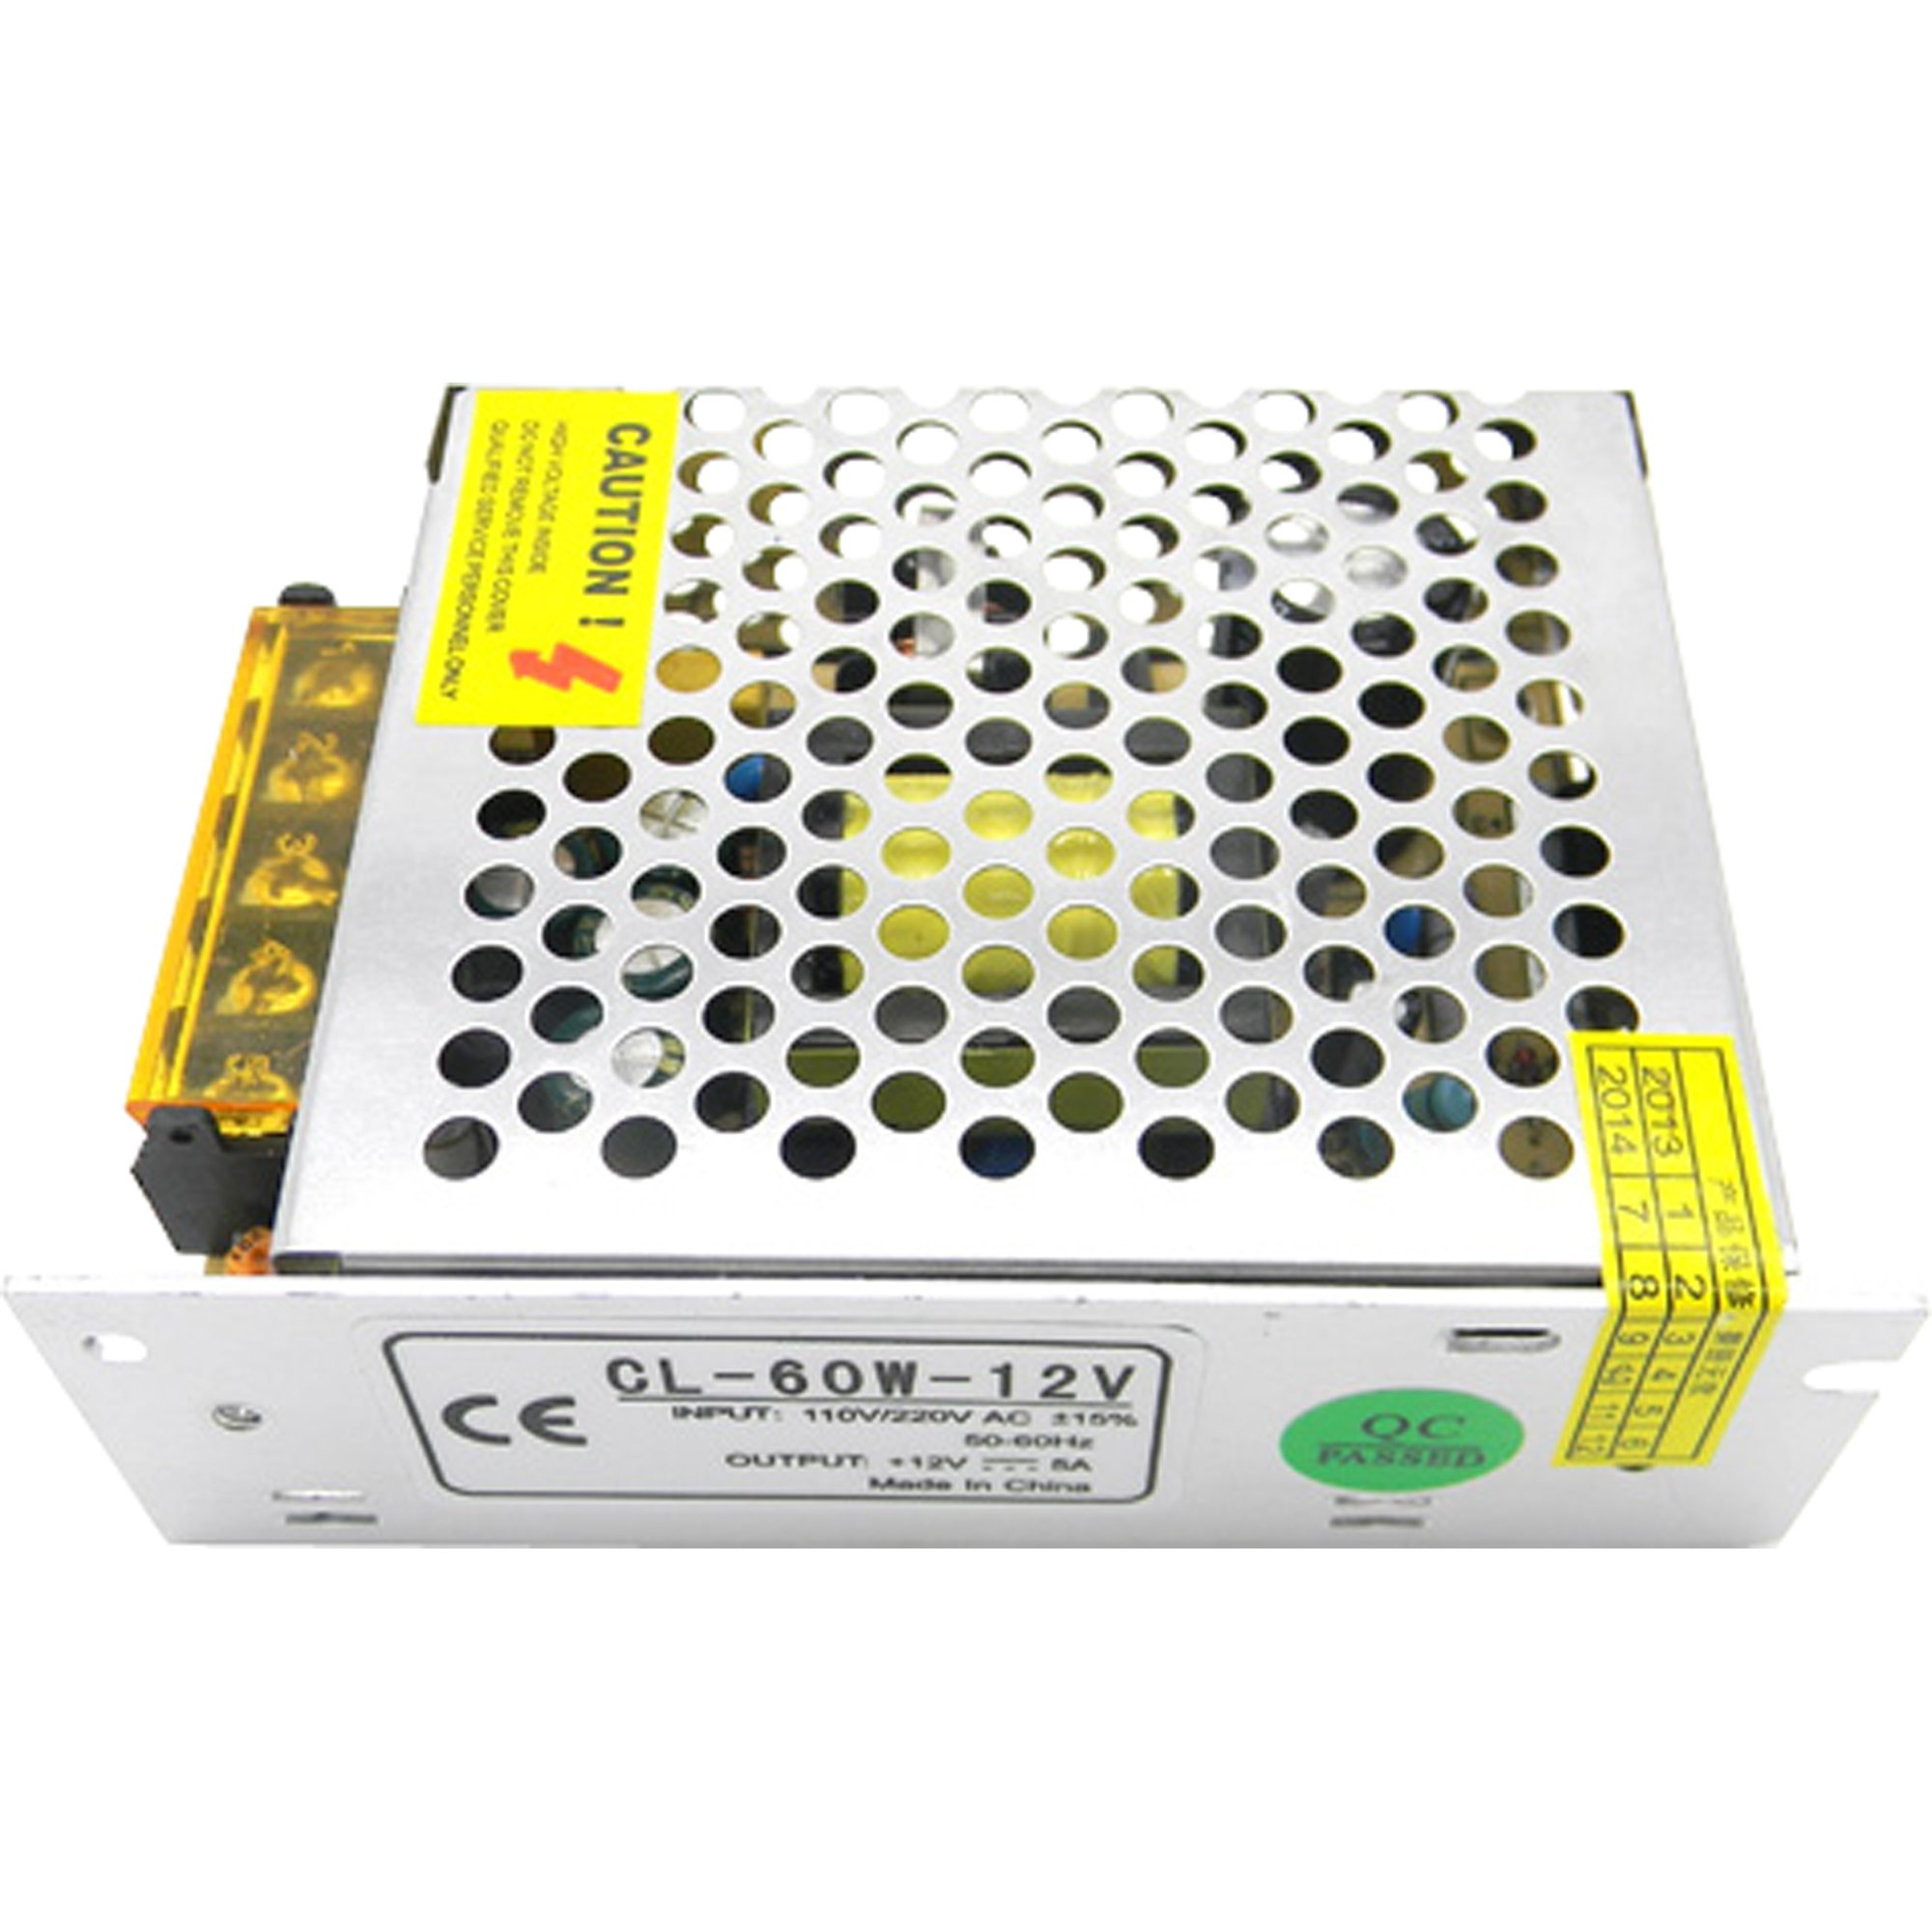
\includegraphics[scale=0.10]{imagens/fonte.jpg}
  	\textsf{\caption{Fonte Colmeia}}
  	\label{fig:FiguraTeste}
\end{figure}

 
\section{Impressão 3D}

    As impressoras 3D estão conquistando espaço no mercado tecnológico, apresentando cada vez mais novidades, como a impressão de brinquedos e a fabricação de tecidos humanos, que no futuro poderá ajudar pacientes que precisam de um implante. As principais peças do robô foram feitas com o auxilio da impressora Void 3D, essa máquina constrói peças funcionais e bastante resistentes.
    
\section{Construção das Peças}


As peças que foram criadas com o auxílio da impressora são: o braço mecânico, a base para o cubo e a placa na qual está disposta os outros componentes.
Os objetos são impressos através da adição de camadas sobrepostas até ser moldado na forma final. O objeto a ser impresso deve ser, primeiramente, desenvolvido em um computador. Após criar o modelo tridimensional é necessário inseri-lo no software da impressora definindo as dimensões da imagem. O software da impressão irá compilar todos os dados e sistematizar em várias camadas. Em seguida inicia-se a impressão. Nesta etapa, na medida que o material derrete, ele é injetado em uma base, que se movimenta em dois eixos e cria as camadas. O processo então é feito camada por camada, desta forma, quando uma fica pronta, outra se inicia até que o objeto fique totalmente pronto. Os materiais mais comuns utilizados nas impressoras 3D são o plástico ABS (ou Acrilonitrila Butadieno Estireno). Este tipo de polímero é bastante rígido e leve, apresentando um bom equilíbrio entre resistência e flexibilidade e o PLA (ácido poliático), que é um polímetro biodegradável, produzido a partir de ácido láctio fermentado a partir de culturas.\cite{impressora}




